\documentclass[10pt,compress]{beamer}
\usepackage[utf8]{inputenc}          % UTF-8 Encoding
\usepackage{hyperref}                % Interactive PDF
\usepackage{listings}
\usepackage[T1]{fontenc}
\usepackage{lmodern}

% Listing layout
\lstdefinestyle{spacey}{
    basicstyle=\ttfamily\small,
    breakatwhitespace=false,         
    breaklines=true,                 
    captionpos=b,                    
    keepspaces=true,                 
    numbers=none,                    
    numbersep=5pt,                  
    showspaces=false,                
    showstringspaces=false,
    showtabs=false,                  
    tabsize=2,
    escapeinside={(*}{*)}
}

% Layout
\useinnertheme[sectionpage=none]{metropolis}
\useoutertheme[numbering=fraction]{metropolis}
\usetheme[everytitleformat=regular]{m}
\metroset{block=fill}

%% Hide navigation buttons
\beamertemplatenavigationsymbolsempty

%% Meta-stuff like authors, title, etc.
\author[Daniel Hillerström]{Daniel Hillerström\\\footnotesize{\href{mailto:daniel.hillerstrom@ed.ac.uk}{daniel.hillerstrom@ed.ac.uk}}\\\footnotesize{\href{http://homepages.inf.ed.ac.uk/s1467124}{http://homepages.inf.ed.ac.uk/s1467124}}}
\institute[University of Edinburgh]{CDT Pervasive Parallelism, University of Edinburgh}
\date{\today}
\title{Effective Concurrency} % Just some title; change at a later point.
\subtitle{Pervasive Parallelism Presentation}

% The document
\begin{document}
  \maketitle
  % Input the content

  \begin{frame}
    \frametitle{Different concurrent programming models}
    \textbf{Message-passing programming (distributed memory)}
    \begin{itemize}
      \item MPI
      \item Erlang
    \end{itemize}
    \textbf{Multi-threaded programming (shared memory)}
    \begin{itemize}
      \item OpenMP
      \item Java
    \end{itemize}
    \textbf{Partition Global Address Space programming (hybrid)}
    \begin{itemize}
      \item Coarray Fortran
      \item Unified Parallel C
    \end{itemize}
    \emph{\tiny{This is not a complete picture!}}
  \end{frame}

  \begin{frame}
    \frametitle{Combining concurrency models}
    Different concurrency models are tailored for particular idioms
    \begin{description}
      \item[\alert<1->{MPI}] Process-centric; interaction among processes across many machines.
      \item[\alert<1->{OpenMP}] Thread-centric; interaction between cores on a chip.
    \end{description}
    Sometimes it makes sense to combine different concurrency models.
  \end{frame}

  % Slide 3
  \begin{frame}
    \frametitle{Commonalities}
    \begin{center}
      \begin{figure}
        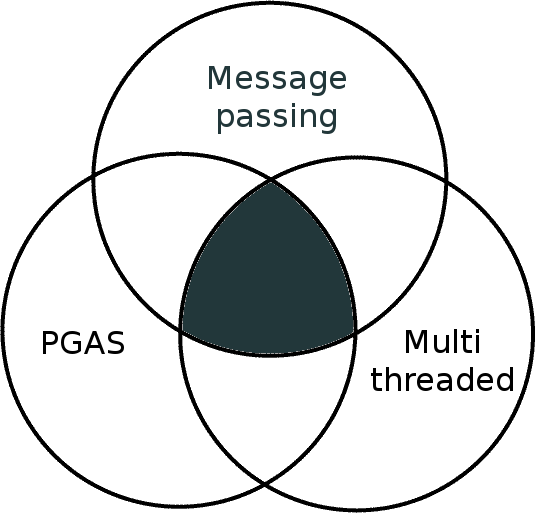
\includegraphics[scale=0.3]{venn.png}
      \end{figure}
    \end{center}
    \uncover<2->{What is the proper abstraction?}

    \emph{\tiny{This is not a complete picture!}}
  \end{frame}

  \begin{frame}
    \frametitle{Problems definition}
    \begin{block}{Problem statement}
      \emph{How can we achieve flexible, composable concurrent programming models, i.e. how can we abstract over the choice of concurrency model?}
    \end{block}
  \end{frame}

  \begin{frame}
    \frametitle{Proposed solution (I)}
    \begin{definition}[Effect]
      An effect is a static description of the potential run-time behaviour of a computation.
    \end{definition}
    Observation:
    \begin{itemize}
      \item Spawning a thread is an effectful computation
      \item Sending a message is an effectful computation
      \item Launching a kernel is an effectful computation
    \end{itemize}
  \end{frame}

  \begin{frame}
    \frametitle{Proposed solution (II)}
    \begin{definition}[Effect handler]
      An effect handler interprets effects.
    \end{definition}
    Observation:
    \begin{itemize}
      \item Modular and compositional approach to modelling effectful computations.
      \item The programmer interpret effects.
      \item It is well-known that handlers can encode concurrency\dots
      \item \dots thus we can separate concurrent computations from their concrete run-time model.
    \end{itemize}
  \end{frame}

  \begin{frame}[containsverbatim]
    \frametitle{Handlers}
    \begin{columns}
      \begin{column}{0.5\textwidth}
Exception handler
\begin{lstlisting}[style=spacey]
  try
    if (n == 0) {
       throw DivZero
    } else {
       m / n
    }
  with
   case DivZero -> 0
\end{lstlisting}        
      \end{column}
      \begin{column}{0.5\textwidth}
Effect handler        
\begin{lstlisting}[style=spacey]
  handle
    if (n == 0) {
       throw (*\alert<1->{DivZero}*)
    } else {
       m / n
    }
  with
   case (*\alert<1->{DivZero}*) (*\alert<1->{k}*) -> 0
   case Return x -> x
\end{lstlisting}    
      \end{column}
    \end{columns}
\tiny{Example adapted from Keuchel and Schrijvers (2014)}
  \end{frame}

  \begin{frame}
    \frametitle{Delimited continuations}
    Delimited continuation
    \begin{itemize}
      \item Looks into the future; multiple invocations.
      \item Returns to the past with the future.
    \end{itemize}
    Powerful, but expensive!
  \end{frame}

  \begin{frame}
    \frametitle{Main idea}
    Optimise handlers based on their invocations of continuations
    \begin{description}
      \item[\alert<1->{Zero times}] No need to allocate space for the continuation.
      \item[\alert<1->{One time}] Recycle allocated space.
      \item[\alert<1->{Multiple times}] Maybe there exists some clever encoding.
    \end{description}
    Track this information in the type system; specialise handlers during code generation.
  \end{frame}

  % Aims and objectives
  \begin{frame}
    \frametitle{Aims and objectives}
    The aim is to implement an (optimizing) compiler for Links.
    \begin{itemize}
       \item Efficient implementation of handlers.
       \item Concurrency for ``free'' through handlers.
    \end{itemize}
  \end{frame}

  \begin{frame}
    \frametitle{Project feasibility}
    \begin{table}
      \centering
      \begin{tabular}{| l | l | l|}
        \hline
        Language & Risk   & Fun \\
        \hline
        Frank    & Medium & {\color{red}{High}} \\
        \hline
        Koka     & {\color{red}{High}}   & {\color{red}{High}} \\
        \hline
        Eff      & {\color{red}{High}}   & {\color{red}{High}} \\
        \hline
        OCaml    & {\color{red}{High}}   & {\color{red}{High}} \\
        \hline
        Links    & {\color{green}{Low}}    & Medium \\
        \hline
      \end{tabular}
      \caption{Risk analysis}
    \end{table}
  \end{frame}

  \begin{frame}
    \frametitle{Colleagues}
    \only<2-2>{Q: Researching efficient handlers?}
    \only<3-3>{Q: Perspective to concurrency/parallelism?}
    \only<4-4>{Q: Using resource-tracking type system to optimise handlers?}
    \begin{table}
      \centering
      \begin{tabular}{| l | l |}
        \hline
        Who  & Work\\
        \hline
        \only<1-1>{Plotkin and Pretnar & Discovers; Handling Algebraic Effects \\
        \hline
        Bauer and Pretnar   & Eff language \\       
        \hline
        McLaughlin, Lindley and McBride & Frank \\
        \hline}
        \only<1-2>{Schrijvers and Wu   & Fusion for Free; Scoped Handlers \\
        \hline}
        \only<1-3>{OCaml Labs          & Multicore OCaml \\
        \hline}
        Hillerström         & Links with Effect Handlers\\
        \hline
      \end{tabular}\caption{Implementators}
    \end{table}
  \end{frame}
  
  % Evaluation
  \begin{frame}
    \frametitle{Evaluation}
    Collection of micro-benchmarks
    \begin{itemize}
      \item Sanity checks
      \item Already written
    \end{itemize}
    Collection of performance benchmarks
    \begin{itemize}
      \item Measuring the feasibility of my implementation
      \item Building the benchmark suite from PLDI\dots
    \end{itemize}
  \end{frame}

  \begin{frame}
    \frametitle{In summary}
    Goals
    \begin{itemize}
      \item Efficient implementation of handlers.
      \item Examine the feasibility of handler-encoded concurrency.
      \item Application: Combine (a restricted subset of) different models (e.g. MPI \& OpenMP)
    \end{itemize}
  \end{frame}

  % Bibliography
  \nocite{*}
  \bibliographystyle{unsrt}
  \begin{frame}[allowframebreaks]
    \frametitle{References}
    \bibliography{references}
  \end{frame}
\end{document}

